\documentclass{exam}

\usepackage{units} 
\usepackage[fleqn]{amsmath}
\usepackage{float}
\usepackage{mdwlist}
\usepackage{booktabs}
\usepackage{caption}
\usepackage{fullpage}
\usepackage{enumerate}
\usepackage{graphicx}

% \usepackage{2in1, lscape} 

\everymath{\displaystyle}
\setcounter{tocdepth}{2}
\printanswers

\newcommand*\mean[1]{\overline{#1}}

\author{}
\date{January 22, 2014}
\title{Statistics \\ Week One}

\begin{document}

  \maketitle
  \tableofcontents

  \pagebreak

  \part{Describing Shape Numerically}

  \section{Overview}

  \begin{itemize}
    \item describing pile of samples like describing pile of rocks:
      \begin{itemize*}
        \item center (median or mean)
        \item number of rocks
        \item shape
      \end{itemize*}

    \item mean vs. median tax cut from {\em Proofiness}

  \end{itemize}

  \subsection{Data}
  (8, 2, 7, 4, 12, 4, 5, 3, 13, 4, 8, 17, 13, 20, 2)

  \section{Central Tendency}

  \subsection{Mean}

  \begin{itemize*}
    \item add up all the numbers and divide by count

    \item center of gravity if the histogram was placed on a weightless plank

    \item sensitive to outliers (Bill Gates walks into a bar)

    \item good for symmetric distributions

    \item stable--if you grab different samples from a large data set, you'll usually get
      the same mean.

    \item used to calculate other statistics like Standard Deviation
  \end{itemize*}

  For sample data, mean is 8.133

  \subsection{Median}

  \begin{itemize*}
    \item middle number, with odd number of samples

    \item mean of two middle numbers with even number of samples

    \item split histogram into two equal area regions

    \item insensitive to outliers (Bill Gates walks into a bar probably doesn't change the
      median much)

    \item unstable--if you grab different samples from a large data set, you may see
      variations in the median.

    \item used to calculate other statistics like Standard Deviation
  \end{itemize*}

  For sample data, median is 7

  \section{Spread/Shape}
  \subsection{Standard Deviation}

  The standard deviation describes the ``average'' distance from the mean.

  \subsubsection{Simple Average Distance}
  \begin{align*}
    \frac{1}{n} \sum (x_i - \mean{x}) & = \sum \frac{x_i}{n} - \sum \frac{ \mean{x} }{n} \\
                                      & = \sum \frac{x_i}{n} - \mean{x} \\
                                      & = \mean{x} - \mean{x} \\
                                      & = 0 \\
  \end{align*}

  \subsubsection{Average Deviation}
  \[
    p = \frac{1}{n} \sum |x_i - \mean{x}|
  \]

  \subsubsection{Variance}
  \[
    s^2 = \frac{1}{n - 1} \sum ( x_i - \mean{x} )^2
  \]

  \subsubsection{Standard Deviation}
  \[
    s = \sqrt{s^2}
  \]

  \begin{itemize*}
    \item shows spread around mean---use in conjunction with the mean
    \item $s^2 \geq 0$
    \item same units as measurement
    \item not resistant---sensitive to outliers
  \end{itemize*}

  For sample data, $s^2 = 5.64$

  \subsection{Quartiles}

  \begin{itemize*}
    \item median of samples above/below the median
    \item used in conjunction with the mean
    \item unstable
    \item resistant
    \item Inter-Quartile Range is difference between third and first quartile
    \item outliers are more than 1.5 IQR from mean
  \end{itemize*}

  \begin{table}[ht]
    \centering
    \begin{tabular}{rrrrrrr}
      \toprule
      \midrule
        & Min. & 1st Qu. & Median & Mean & 3rd Qu. & Max. \\
      1 & 2.00 & 4.00    & 7.00   & 8.13 & 12.50   & 20.00 \\
      \bottomrule
    \end{tabular}
  \end{table}

  \section{Exercises}

  \begin{enumerate}
    \item Can $s^2$ ever be larger than $\mean{x}$?

      \begin{solution}
        sure.  For example (1, 1, 16) has mean of 6 and $s^2 \approx 8.66$
      \end{solution}

    \item Which list has largest $s^2$?
      \begin{itemize*}
        \item (0, 20, 40, 50, 60, 80, 100) ($s^2 = 28.6$)
        \item (0, 48, 49, 50, 51, 52, 100) ($s^2 = 28.9$)
        \item (0, 1, 2, 50, 98, 99, 100) ($s^2 = 49.0$)
      \end{itemize*}

    \item One investigator takes a sample of 100 men and another takes a sample of 1000 men. 
      \begin{itemize*}
        \item Is either investigator more likely to get the largest mean? (no)
        \item Is either investigator more likely to get the largest $s^2$? (no)
        \item Is either investigator more likely to get the tallest? (bigger sample, bigger
          range)
        \item Is either investigator more likely to get the shortest? (bigger sample, bigger
          range)
      \end{itemize*}

    \item 
      \begin{parts}
        \part
          If everyone in a company got a \$1,000 raise, what would this do to the mean wage and
          the standard deviation?

          \begin{solution}
            Average wage goes up by \$1000, standard deviation doesn't change.

            \begin{align*}
              \mean{x}_{new} & = \frac{1}{n} \sum (x_i + 1000) \\
                             & = 1000 + \mean{x}_{old} \\
            \end{align*}

            For standard deviation, in each term, the mean goes up by \$1,000 and $x_i$ goes up by
            \$1000 so there is no net change.

          \end{solution}

        \part 
          If everyone in the company got a 5\% raise, what would this do to the mean wage and the
          standard deviation?

          \begin{solution}
            Both go up by 5\%

            \begin{align*}
              \mean{x}_{new} & = \frac{1}{n} \sum (1.05 x_i) \\
                             & = 1.05 \mean{x}_{old} \\
            \end{align*}

            Similarly for $s^2$.

          \end{solution}

      \end{parts}

  \end{enumerate}

  \pagebreak

  \part{NFL}

  \section{Overview}
  First eight Seahawks games of 2012.

  \section{Passing Sample}

  \subsection{Data}
  \begin{table}[H]
    \centering
    \begin{tabular}{rllr}
      \toprule
          & PSR     & TRG     & YDS \\
      \midrule
      96  & RW-3850 & DB-0500 & 10 \\
      129 & RW-3850 & GT-0100 & -6 \\
      53  & RW-3850 & AM-1400 & 5 \\
      149 & RW-3850 & SR-0500 & 0 \\
      154 & RW-3850 & DB-0500 & 7 \\
      144 & RW-3850 & ZM-0200 & 7 \\
      166 & RW-3850 & ZM-0200 & 0 \\
      64  & RW-3850 & GT-0100 & 41 \\
      192 & RW-3850 & LW-0500 & 9 \\
      27  & RW-3850 & BE-0200 & 8 \\
      130 & RW-3850 & DB-0500 & 50 \\
      128 & RW-3850 & ZM-0200 & 22 \\
      32  & RW-3850 & SR-0500 & 0 \\
      43  & RW-3850 & SR-0500 & 18 \\
      163 & RW-3850 & AM-1400 & 0 \\
      \bottomrule
    \end{tabular}
    \caption{Sample of passes}
  \end{table}

  \subsection{All Passes}

  \begin{figure}[H]
    \centering
    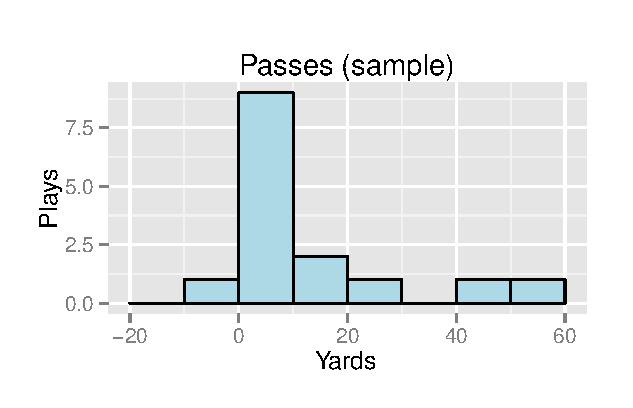
\includegraphics{figures/nfl/sample_passes_histogram.eps}
    \caption{Passes histogram (sample)}
  \end{figure}

  \begin{table}[H]
    \centering
    \begin{tabular}{rlll}
      \toprule
        & PSR        & TRG       & YDS \\
      \midrule
      1 & RW-3850:15 & DB-0500:3 & Min.   :-6.0   \\
      2 & AB-3500: 0 & SR-0500:3 & 1st Qu.: 0.0   \\
      3 & AD-0100: 0 & ZM-0200:3 & Median : 7.0   \\
      4 & AE-0500: 0 & AM-1400:2 & Mean   :11.4   \\
      5 & AL-1100: 0 & GT-0100:2 & 3rd Qu.:14.0   \\
      6 & AR-1300: 0 & BE-0200:1 & Max.   :50.0   \\
      7 & (Other): 0 & (Other):1 & $s^2$  :15.68 \\
      \bottomrule
    \end{tabular}
    \caption{Passes summary (sample)}
  \end{table}

  \begin{figure}[H]
    \centering
    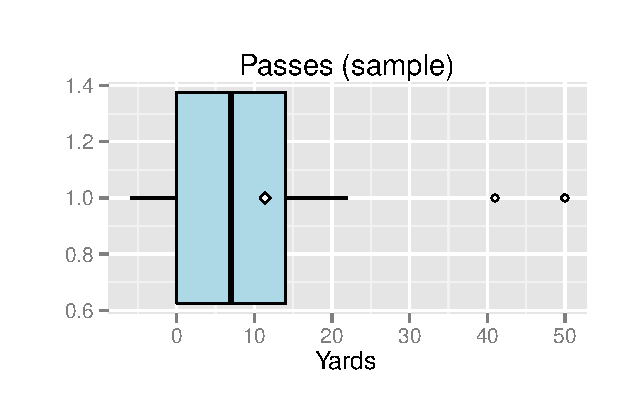
\includegraphics{figures/nfl/sample_passes_box.eps}
    \caption{Passes box chart (sample)}
  \end{figure}

  \subsection{Completions}

  \begin{figure}[H]
    \centering
    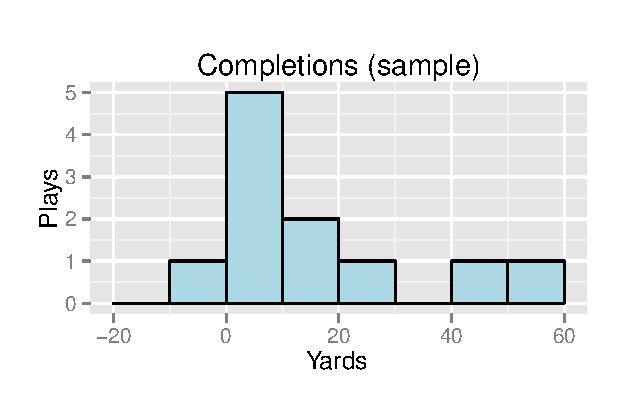
\includegraphics{figures/nfl/sample_completions_histogram.eps}
    \caption{Completions histogram (sample)}
  \end{figure}

  \begin{table}[H]
    \centering
    \begin{tabular}{rlll}
      \toprule
      \midrule
         & PSR        & TRG       & YDS \\
      1  & RW-3850:11 & DB-0500:3 & Min.   :-6.00   \\
      2  & AB-3500: 0 & GT-0100:2 & 1st Qu.: 7.00   \\
      3  & AD-0100: 0 & ZM-0200:2 & Median : 9.00   \\
      4  & AE-0500: 0 & AM-1400:1 & Mean   :15.55   \\
      5  & AL-1100: 0 & BE-0200:1 & 3rd Qu.:20.00   \\
      6  & AR-1300: 0 & LW-0500:1 & Max.   :50.00   \\
      7  & (Other): 0 & (Other):1 & $s^2$  : 16.54 \\
      \bottomrule
    \end{tabular}
    \caption{Completions summary (sample)}
  \end{table}

  \begin{figure}[H]
    \centering
    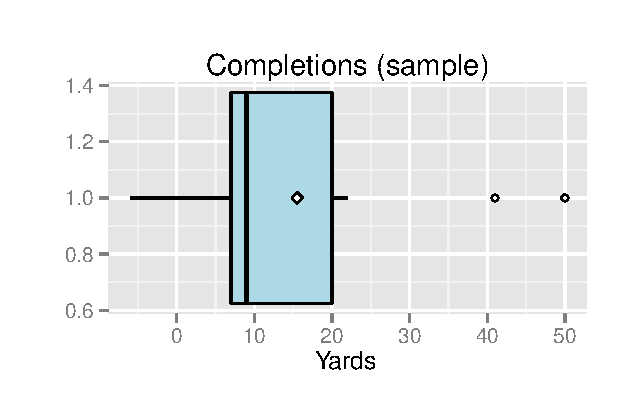
\includegraphics{figures/nfl/sample_completions_box.eps}
    \caption{Completions box (sample)}
  \end{figure}

  \section{Passing vs. Rushing}

  \subsection{Passing}
  \begin{figure}[H]
    \centering
    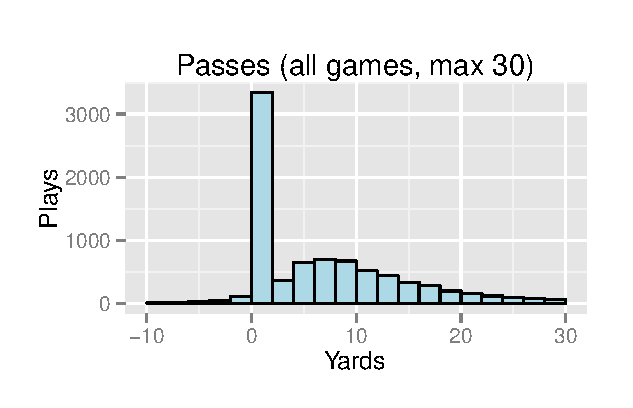
\includegraphics{figures/nfl/passes_histogram.eps}
    \caption{Passing histogram}
  \end{figure}

  \begin{figure}[H]
    \centering
    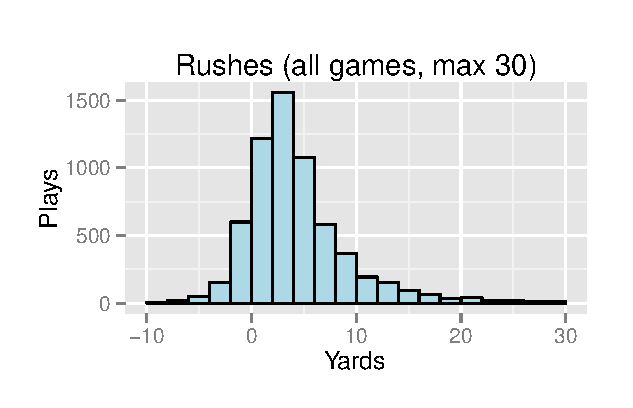
\includegraphics{figures/nfl/rushes_histogram.eps}
    \caption{Rushing histogram}
  \end{figure}

  \begin{figure}[H]
    \centering
    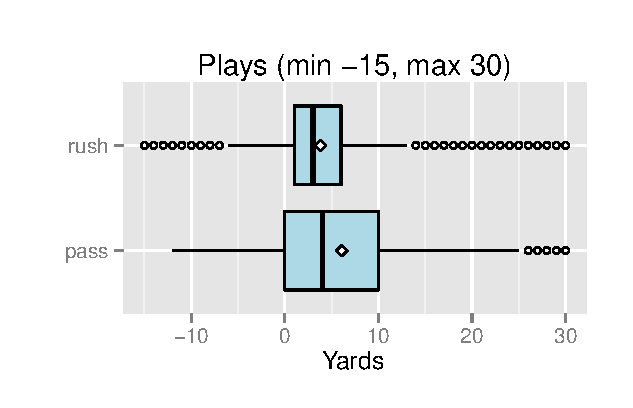
\includegraphics{figures/nfl/rushes_and_passes.eps}
    \caption{All NFL games rushing vs. passing}
  \end{figure}

  % \begin{table}[H]
  %   \centering
  %   \begin{tabular}{rll}
  %     \toprule
  %        & YDS            & TRG \\
  %     \midrule
  %     1  & Min.   :-6.000 & SR-0500:46   \\
  %     2  & 1st Qu.: 0.000 & GT-0100:34   \\
  %     3  & Median : 5.000 & ZM-0200:23   \\
  %     4  & Mean   : 6.952 & DB-0500:19   \\
  %     5  & 3rd Qu.:10.000 & AM-1400:17   \\
  %     6  & Max.   :51.000 & BE-0200:15   \\
  %     7  & $s^2$  : 9.22  & (Other):53   \\
  %     \bottomrule
  %   \end{tabular}
  %   \caption{Passing summary}
  % \end{table}

  % \begin{figure}[H]
  %   \centering
  %   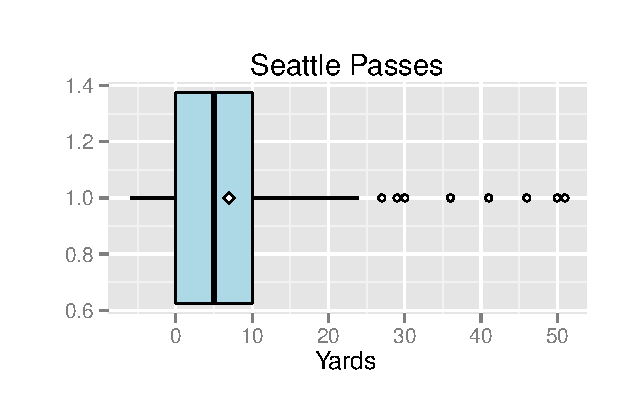
\includegraphics{figures/nfl/passes_box.eps}
  %   \caption{Passes box plot}
  % \end{figure}

  % \begin{table}[H]
  %   \centering
  %   \begin{tabular}{rll}
  %     \toprule
  %       & YDS           & TRG \\
  %     \midrule
  %     1 & Min.   :-6.00 & SR-0500:28   \\
  %     2 & 1st Qu.: 6.00 & GT-0100:20   \\
  %     3 & Median : 9.00 & ZM-0200:16   \\
  %     4 & Mean   :11.41 & DB-0500:11   \\
  %     5 & 3rd Qu.:15.00 & ML-2500:11   \\
  %     6 & Max.   :51.00 & RT-1950:11   \\
  %     7 & $s^2$  : 9.41 & (Other):31   \\
  %     \bottomrule
  %   \end{tabular}
  %   \caption{Completions summary}
  % \end{table}

  % \begin{figure}[H]
  %   \centering
  %   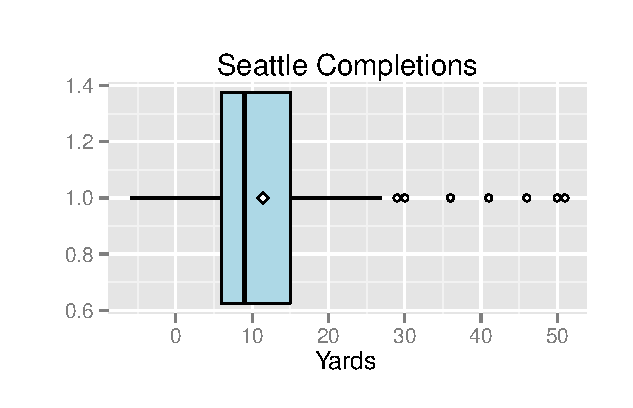
\includegraphics{figures/nfl/completions_box.eps}
  %   \caption{Completions box plot}
  % \end{figure}

  % \subsection{Rushing}


  % \begin{table}[H]
  %   \centering
  %   \begin{tabular}{rlll}
  %     \toprule
  %     \midrule
  %       & YDS            & BC          & DIR \\
  %     1 & Min.   :-18    & ML-2500:159 & LT     :62   \\
  %     2 & 1st Qu.:  2    & RW-3850: 36 & MD     :51   \\
  %     3 & Median :  3    & RT-1950: 30 & RT     :47   \\
  %     4 & Mean   :  4    & LW-0500: 10 & RE     :27   \\
  %     5 & 3rd Qu.:  6    & MR-1500:  6 & LE     :21   \\
  %     6 & Max.   : 77    & JR-3700:  2 & LG     :20   \\
  %     7 & $s^2$  :  6.72 & (Other):  3 & (Other):18   \\
  %     \bottomrule
  %   \end{tabular}
  %   \caption{Seattle rushing summary}
  % \end{table}

  % \begin{figure}[H]
  %   \centering
  %   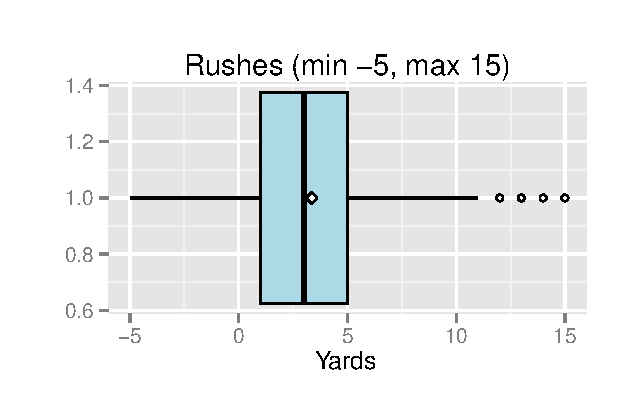
\includegraphics{figures/nfl/rushes_box.eps}
  %   \caption{Seattle rushing box plot}
  % \end{figure}

  \section{Top Rushers}
  \begin{table}[H]
    \centering
    \begin{tabular}{lllllllll}
      \toprule
      \midrule
      BC      & total & sd    & Min. & 1st Qu. & Median & Mean & 3rd Qu. & Max. \\
      AP-0700 & 775   & 7.91  & -4   & 1.00    & 3      & 5.13 & 6.0     & 64 \\
      ML-2500 & 757   & 7.35  & -4   & 2.00    & 3      & 4.76 & 6.0     & 77 \\
      SR-0700 & 718   & 6.30  & -4   & 1.00    & 3      & 4.79 & 7.0     & 41 \\
      AM-2850 & 717   & 6.55  & -4   & 1.00    & 3      & 4.75 & 6.0     & 39 \\
      AF-0900 & 659   & 5.40  & -4   & 1.00    & 3      & 3.92 & 5.0     & 46 \\
      FG-0200 & 654   & 6.50  & -4   & 1.75    & 4      & 5.45 & 7.0     & 37 \\
      JC-2300 & 599   & 11.21 & -11  & 0.00    & 3      & 5.03 & 6.5     & 91 \\
      CJ-1700 & 595   & 8.75  & -8   & 1.00    & 3      & 4.54 & 6.0     & 83 \\
      AB-2600 & 570   & 6.13  & -5   & 1.00    & 3      & 4.52 & 5.0     & 37 \\
      WM-0300 & 554   & 5.00  & -4   & 2.00    & 3      & 4.50 & 6.0     & 31 \\
      DM-0450 & 543   & 6.11  & -4   & 1.00    & 3      & 4.21 & 5.0     & 41 \\
      RR-0400 & 524   & 6.58  & -4   & 1.00    & 3      & 4.94 & 6.0     & 43 \\
      CS-3400 & 523   & 10.50 & -5   & 2.00    & 5      & 7.26 & 8.0     & 56 \\
      SG-1300 & 509   & 4.57  & -6   & 1.00    & 3      & 3.66 & 5.0     & 36 \\
      LM-1000 & 502   & 5.80  & -6   & 0.00    & 3      & 3.95 & 6.5     & 34 \\
      RB-4900 & 493   & 7.88  & -9   & 1.00    & 3      & 4.40 & 6.0     & 65 \\
      RG-1850 & 479   & 10.54 & -7   & 3.00    & 6      & 7.15 & 9.0     & 76 \\
      TR-0350 & 470   & 4.82  & -3   & 1.00    & 3      & 3.70 & 5.0     & 32 \\
      DM-1600 & 438   & 7.12  & -11  & 1.00    & 2      & 3.32 & 4.0     & 64 \\
      MF-1300 & 436   & 6.09  & -3   & 1.00    & 3      & 4.59 & 6.0     & 39 \\
      \bottomrule
    \end{tabular}
  \end{table}

  \begin{figure}[H]
    \centering
    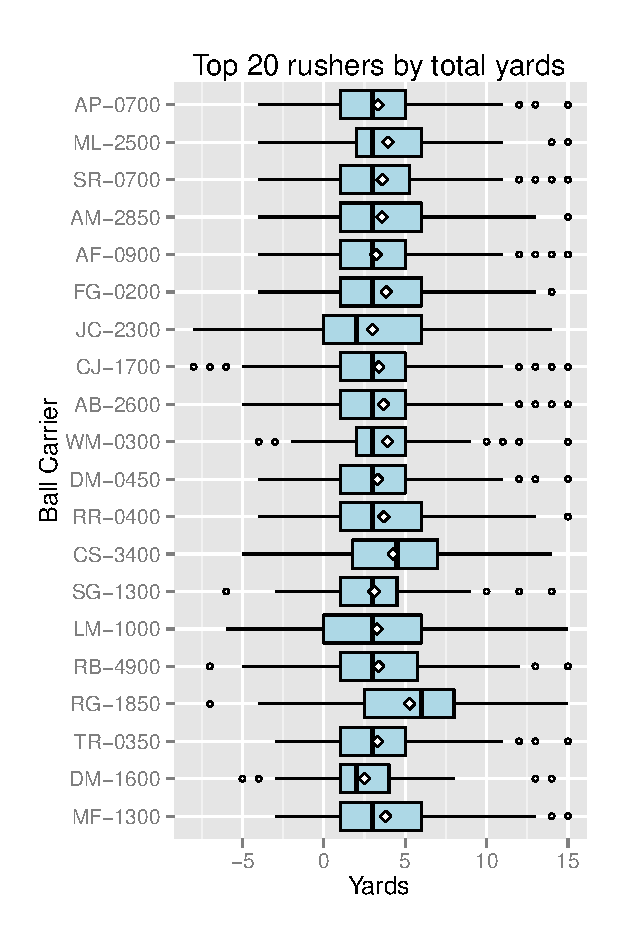
\includegraphics{figures/nfl/top_rushers.eps}
    \caption{Top 20 rushers by total yards}
  \end{figure}

  \part{Income and Education}

  \section{Sample Data}

  \begin{table}[H]
    \centering
    \begin{tabular}{rlllr}
      \toprule
        ID & Education         & Sex   & Race   & Wages \\
      \midrule
         1 & HS or GED         & Black & Female & 35,000 \\
         2 & HS or GED         & Asian & Female & 30,000 \\
         3 & Master's Degree   & White & Male   & 180,000 \\
         4 & HS or GED         & White & Male   & 92,000 \\
         5 & Some College      & Asian & Female & 80,000 \\
         6 & Some College      & White & Female & 32,000 \\
         7 & Some College      & White & Male   & 65,000 \\
         8 & No HS Diploma     & White & Male   & 22,000 \\
         9 & Bachelor's Degree & White & Male   & 57,000 \\
        10 & Some College      & White & Female & 20,000 \\
      \bottomrule
    \end{tabular}
  \end{table}

  \begin{table}[ht]
    \centering
    \begin{tabular}{rrrrrrrr}
      \toprule
        Std Dev & Min.  & 1st Qu. & Median & Mean  & 3rd Qu. & Max. \\
      \midrule
        48527   & 20000 & 30500   & 46000  & 61300 & 76250   & 180000 \\
      \bottomrule
    \end{tabular}
  \end{table}

  \section{Wages}

  \subsection{Overall}
  \begin{figure}[H]
    \centering
    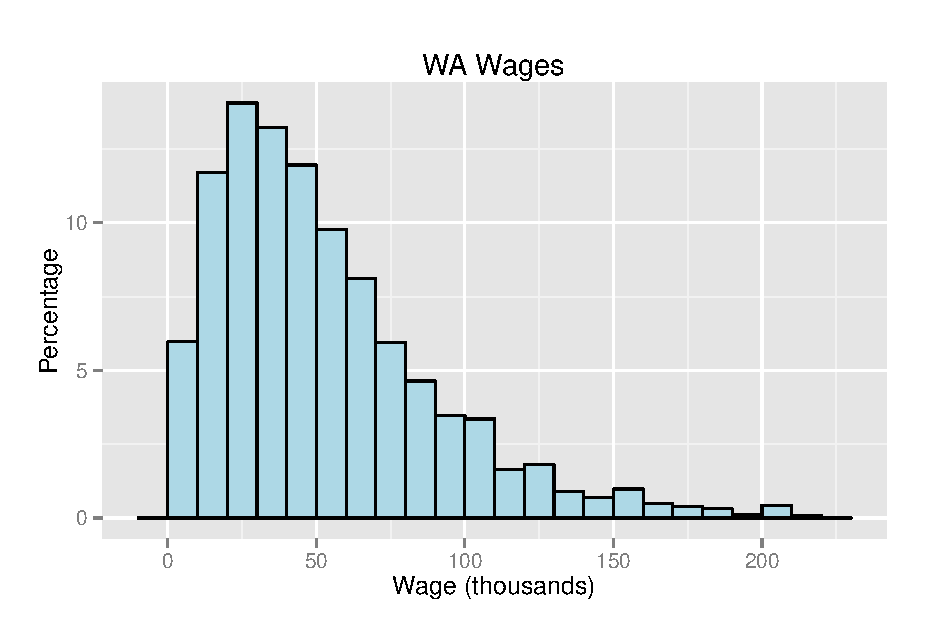
\includegraphics[scale = 0.8]{figures/wa_wage_histogram.eps}
    \caption{WA wage histogram}
  \end{figure}

  \begin{figure}[H]
    \centering
    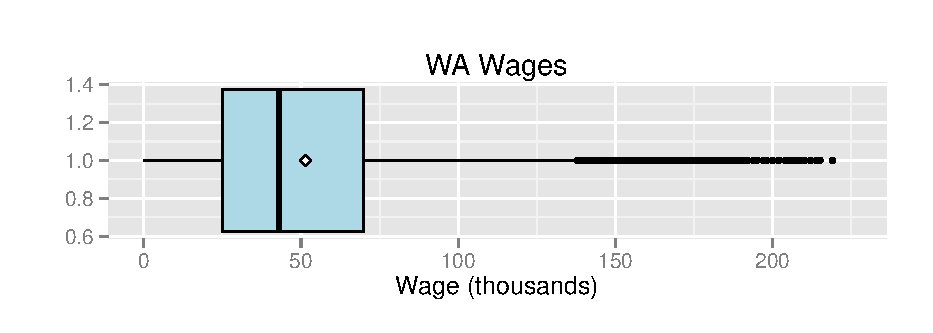
\includegraphics{figures/wa_wage.eps}
    \caption{WA wage box plot}
  \end{figure}

  \begin{table}[ht]
    \centering
    \begin{tabular}{rrrrrrrrr}
      \toprule
        Count & Std Dev & 1st Qu. & Median & Mean  & 3rd Qu. & Max. \\
      \midrule
        24388 & 36689   & 24200   & 42300  & 51240 & 70000   & 219000 \\
      \bottomrule
    \end{tabular}
  \end{table}

  \subsection{By Race}
  \begin{figure}[H]
    \centering
    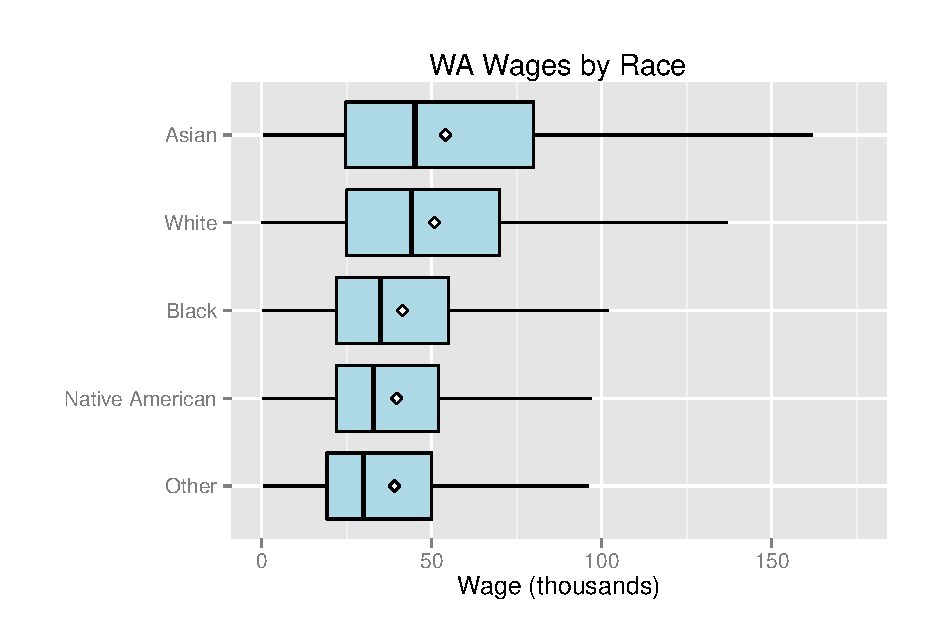
\includegraphics{figures/wa_wage_by_race.eps}
    \caption{WA wages by race}
  \end{figure}

  \begin{table}[ht]
    \centering
    \begin{tabular}{rlrrrrrrrr}
      \toprule
          & race   & Count & Std Dev & Min. & 1st Qu. & Median & Mean  & 3rd Qu. & Max. \\
      \midrule
        1 & Asian  & 1786  & 40247   & 600  & 25000   & 45000  & 55780 & 80000   & 215000 \\
        2 & Black  & 667   & 30004   & 360  & 22000   & 35000  & 41790 & 55000   & 187000 \\
        3 & Native & 498   & 28512   & 100  & 22000   & 33000  & 40640 & 52750   & 214000 \\
        4 & Other  & 1402  & 31317   & 430  & 19200   & 30000  & 39950 & 50000   & 219000 \\
        5 & White  & 20035 & 36852   & 30   & 25000   & 44900  & 52200 & 70000   & 219000 \\
      \bottomrule
    \end{tabular}
  \end{table}

  \subsection{By Education}
  \begin{figure}[H]
    \centering
    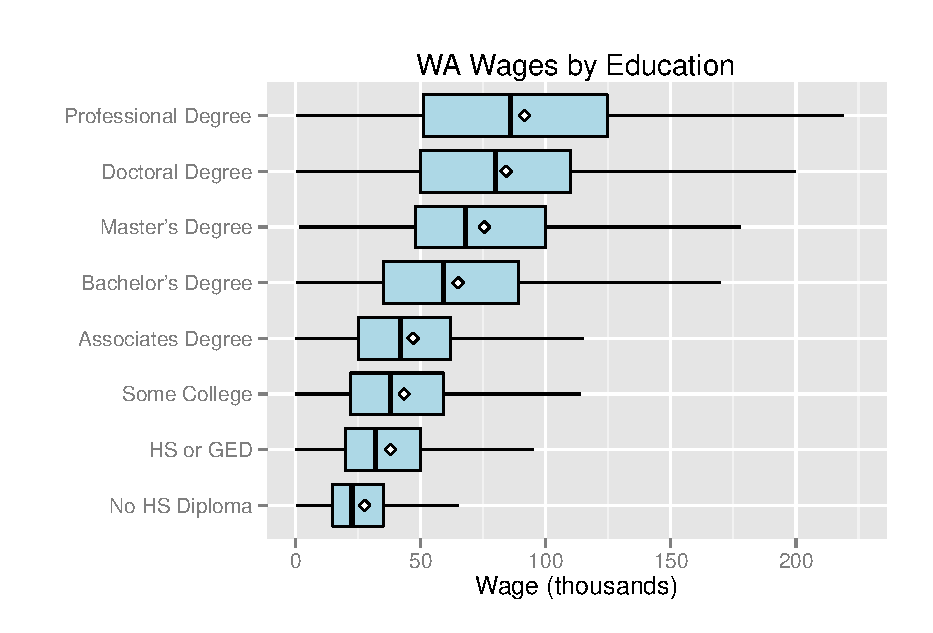
\includegraphics{figures/wa_wage_by_education.eps}
    \caption{WA wages by education}
  \end{figure}

  \begin{table}[ht]
    \centering
    \begin{tabular}{rlrrrrrrrr}
      \toprule
        & education     & Count & Std Dev & Min. & 1st Qu. & Median & Mean  & 3rd Qu. & Max. \\
      \midrule
      1 & Associates    & 2790  & 29158   & 60   & 25000   & 42000  & 46970 & 62000   & 205000 \\
      2 & Bachelor's    & 5687  & 39955   & 380  & 35000   & 59000  & 64930 & 89000   & 215000 \\
      3 & Doctoral      & 368   & 46338   & 200  & 50000   & 80000  & 84110 & 110000  & 212000 \\
      4 & HS or GED     & 5154  & 26030   & 30   & 20000   & 32000  & 37880 & 50000   & 214000 \\
      5 & Master's      & 2230  & 41441   & 1500 & 48000   & 68000  & 75450 & 100000  & 210000 \\
      6 & No HS Diploma & 1471  & 21308   & 330  & 14850   & 22500  & 27600 & 35000   & 219000 \\
      7 & Professional  & 499   & 52328   & 500  & 51000   & 86000  & 91470 & 124500  & 219000 \\
      8 & Some College  & 6189  & 29779   & 100  & 22000   & 38000  & 43400 & 59000   & 215000 \\
      \midrule
    \end{tabular}
  \end{table}

  \begin{figure}[H]
    \centering
    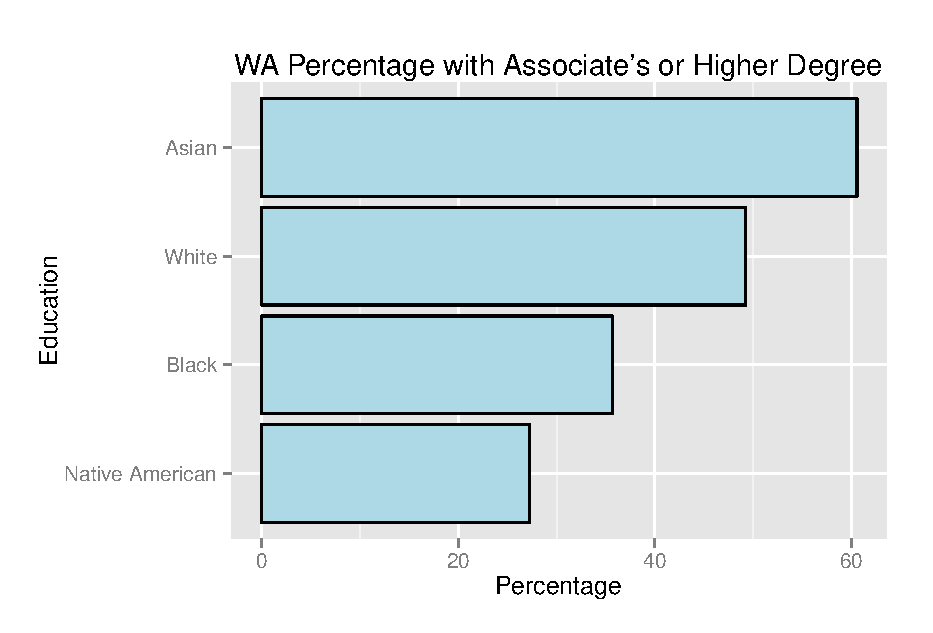
\includegraphics{figures/wa_degree_by_race.eps}
    \caption{Education correlates with wage by race}
  \end{figure}

  \subsection{By Field}
  \begin{figure}[H]
    \centering
    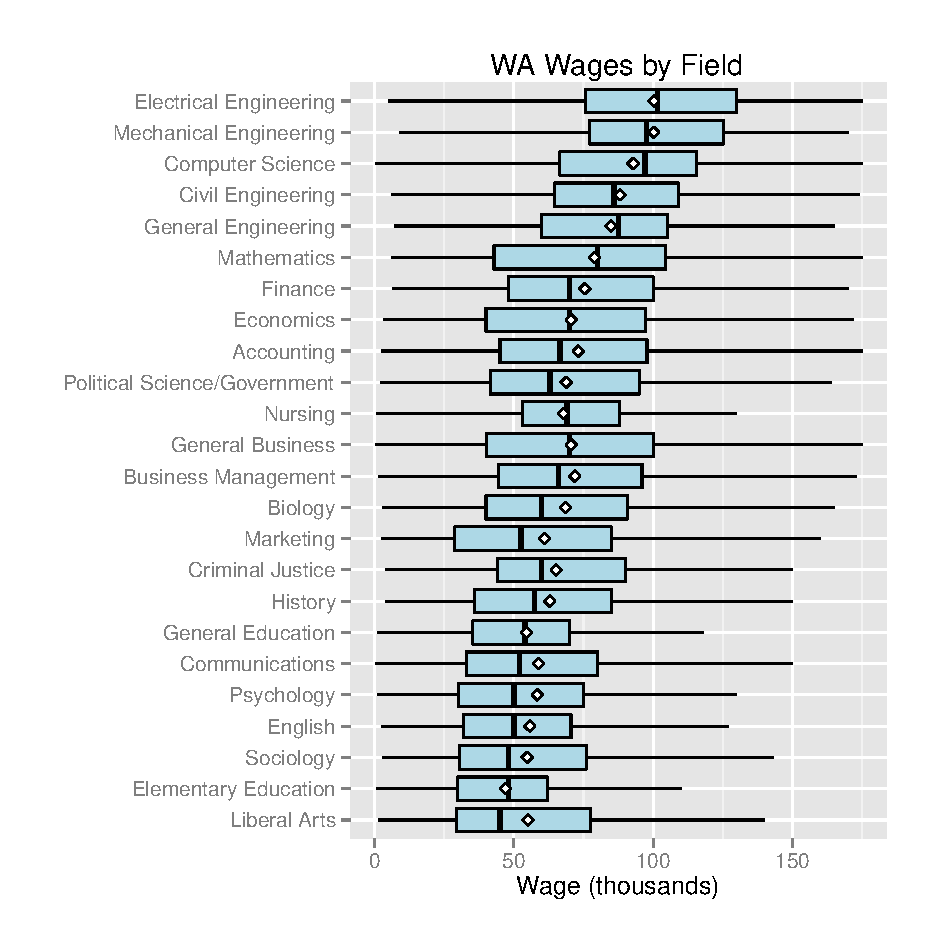
\includegraphics{figures/wa_wage_by_field.eps}
    \caption{WA wages by field}
  \end{figure}

  \begin{table}[ht]
    \centering
    \begin{tabular}{lrrrrrrrr}
      \toprule
      \midrule
      Field                & Count & Std Dev & Min. & 1st Qu. & Median & Mean   & 3rd Qu. & Max. \\
      EE                   & 246   & 43522   & 5000 & 80000   & 104000 & 104000 & 135800  & 207000 \\
      ME                   & 204   & 39081   & 8800 & 78000   & 100000 & 103800 & 130000  & 205000 \\
      CS                   & 264   & 43330   & 480  & 70000   & 99500  & 97800  & 120000  & 209000 \\
      Civil Eng.           & 107   & 42577   & 6000 & 65000   & 90000  & 92030  & 115000  & 200000 \\
      General Eng.         & 111   & 43564   & 7000 & 60000   & 90000  & 91620  & 108500  & 200000 \\
      Mathematics          & 114   & 46415   & 6000 & 45150   & 80000  & 81750  & 108800  & 194000 \\
      Finance              & 105   & 48302   & 6500 & 48000   & 73000  & 83280  & 108000  & 206000 \\
      Economics            & 174   & 45074   & 3200 & 42250   & 70000  & 75030  & 100000  & 215000 \\
      General Business     & 293   & 39849   & 400  & 40300   & 70000  & 70580  & 100000  & 175000 \\
      Accounting           & 254   & 45051   & 2500 & 47250   & 69500  & 77820  & 100000  & 207000 \\
      Nursing              & 340   & 30967   & 650  & 53000   & 69500  & 68860  & 89000   & 210000 \\
      Business Management  & 545   & 41093   & 1500 & 45000   & 68000  & 74950  & 100000  & 205000 \\
      Poli Sci             & 200   & 41587   & 2000 & 43500   & 65000  & 71390  & 98500   & 208000 \\
      Biology              & 277   & 48478   & 3000 & 42000   & 64000  & 76270  & 101000  & 219000 \\
      Criminal Justice     & 126   & 34166   & 4000 & 44250   & 60000  & 66260  & 90000   & 200000 \\
      History              & 179   & 39018   & 4000 & 36500   & 58000  & 65090  & 87500   & 210000 \\
      Marketing            & 108   & 45394   & 2500 & 29520   & 56000  & 65680  & 85750   & 210000 \\
      General Education    & 227   & 30902   & 1000 & 35650   & 54000  & 55910  & 70000   & 210000 \\
      Communications       & 219   & 40177   & 380  & 33500   & 52000  & 61350  & 80000   & 200000 \\
      English              & 288   & 34236   & 2600 & 32000   & 50000  & 55710  & 70500   & 175000 \\
      Psychology           & 394   & 41129   & 1200 & 30180   & 50000  & 60420  & 79750   & 212000 \\
      Sociology            & 175   & 35710   & 3000 & 30750   & 48200  & 56290  & 78500   & 190000 \\
      Elementary Education & 204   & 24105   & 600  & 29900   & 48000  & 47010  & 62000   & 120000 \\
      Liberal Arts         & 153   & 38892   & 1500 & 30000   & 45800  & 57010  & 80000   & 200000 \\
      \bottomrule
    \end{tabular}
  \end{table}

  % \begin{figure}[H]
  %   \centering
  %   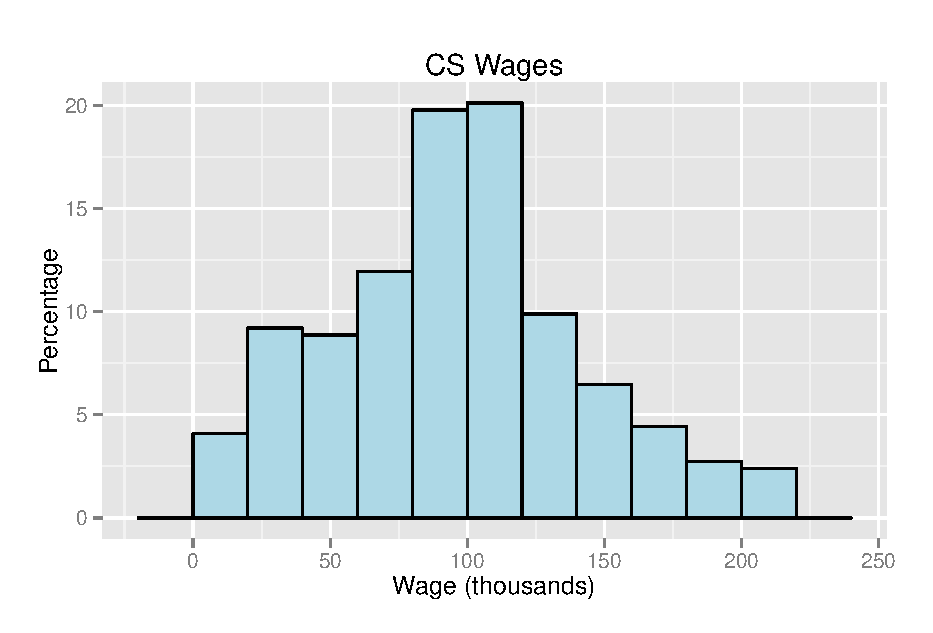
\includegraphics[scale = 0.8]{figures/wa_cs_wages.eps}
  %   \caption{Computer science wage histogram}
  % \end{figure}

  \section{Women vs. Men}

  \begin{figure}[H]
    \centering
    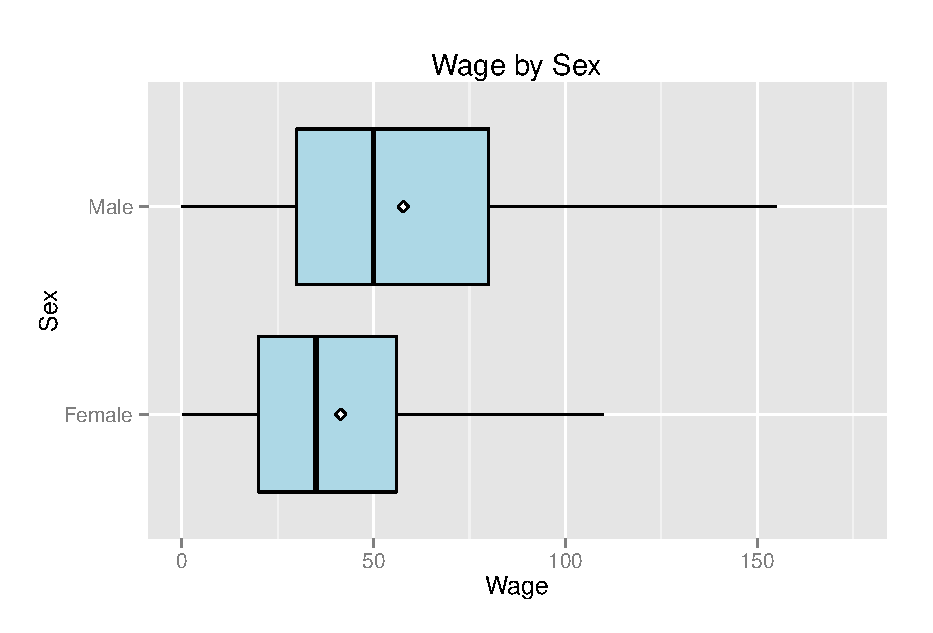
\includegraphics[scale = 0.8]{figures/wa_wage_by_sex.eps}
    \caption{Women make less than men.}
  \end{figure}
  
  \begin{figure}[H]
    \centering
    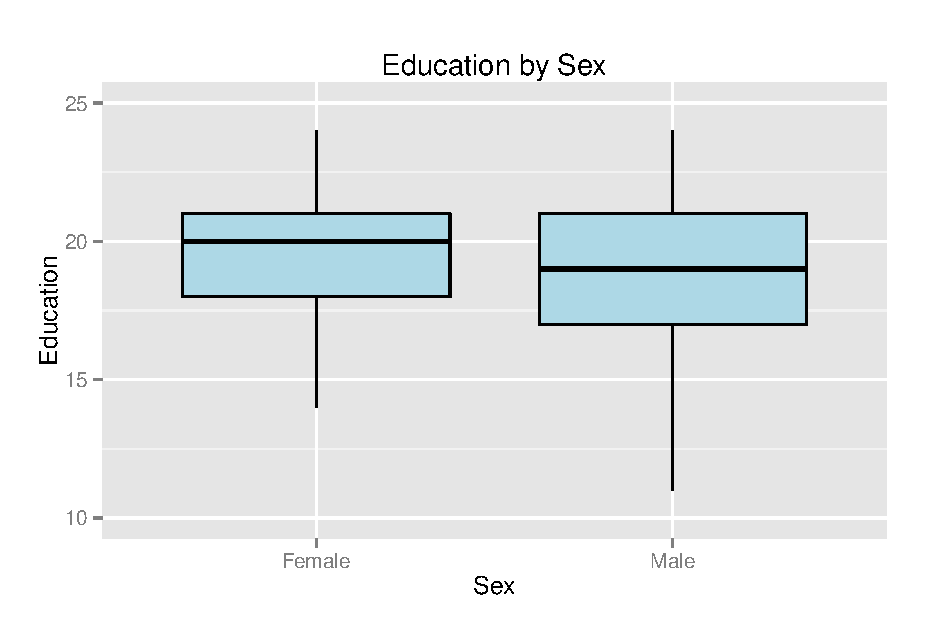
\includegraphics[scale = 0.8]{figures/wa_education_by_sex.eps}
    \caption{Women are a bit more educated than men.}
  \end{figure}

  \begin{figure}[H]
    \centering
    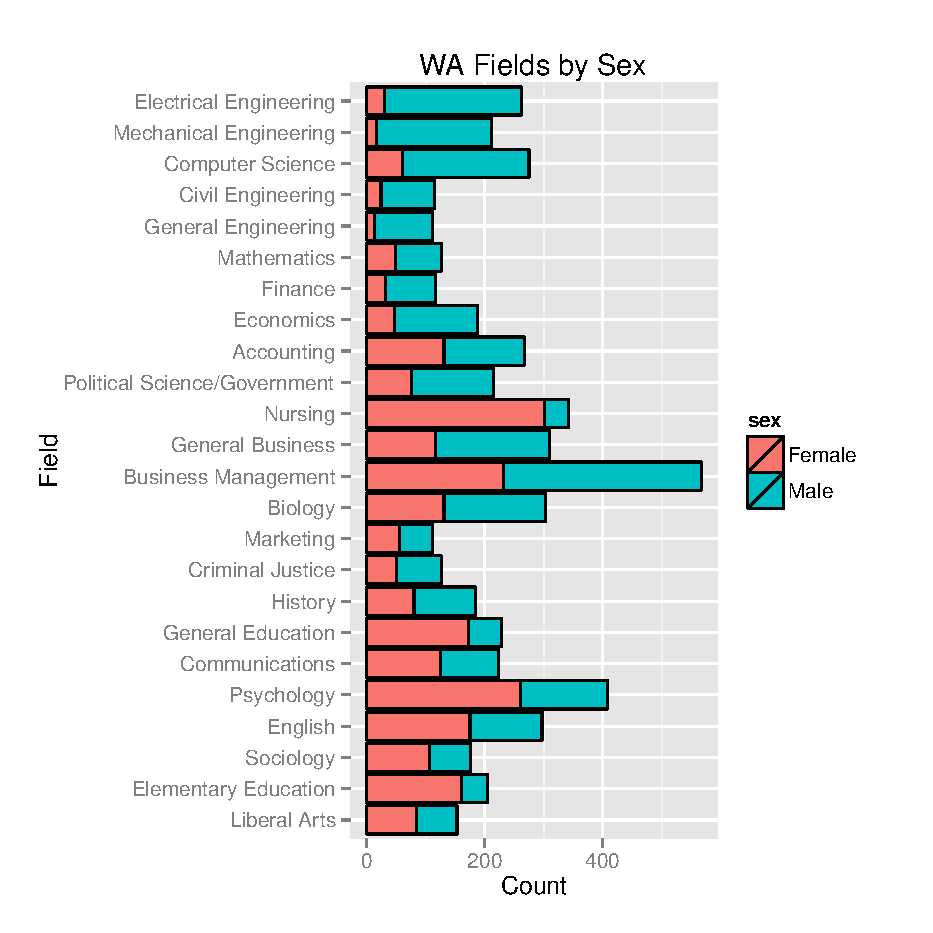
\includegraphics{figures/wa_field_by_sex.eps}
    \caption{ Women tend to get degrees in less lucrative fields.}
  \end{figure}

  
  \begin{figure}[H]
    \centering
    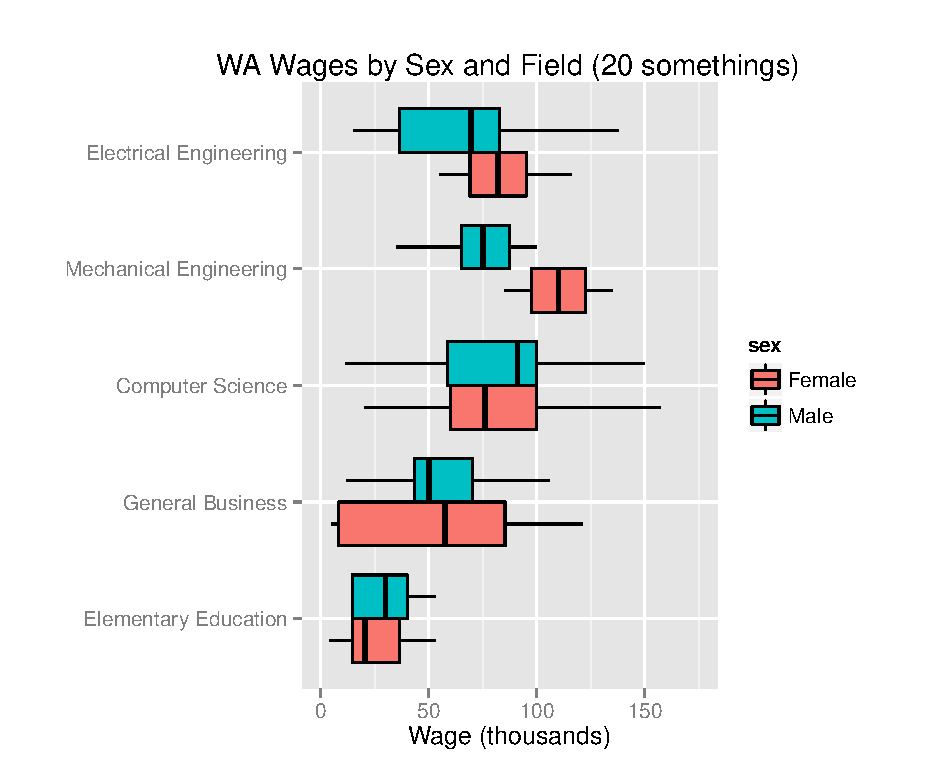
\includegraphics{figures/wa_20s_by_field_and_sex.eps}
    \caption{Twenty to thirty year olds by field seems to be fairly even.}
  \end{figure}

  \begin{figure}[H]
    \centering
    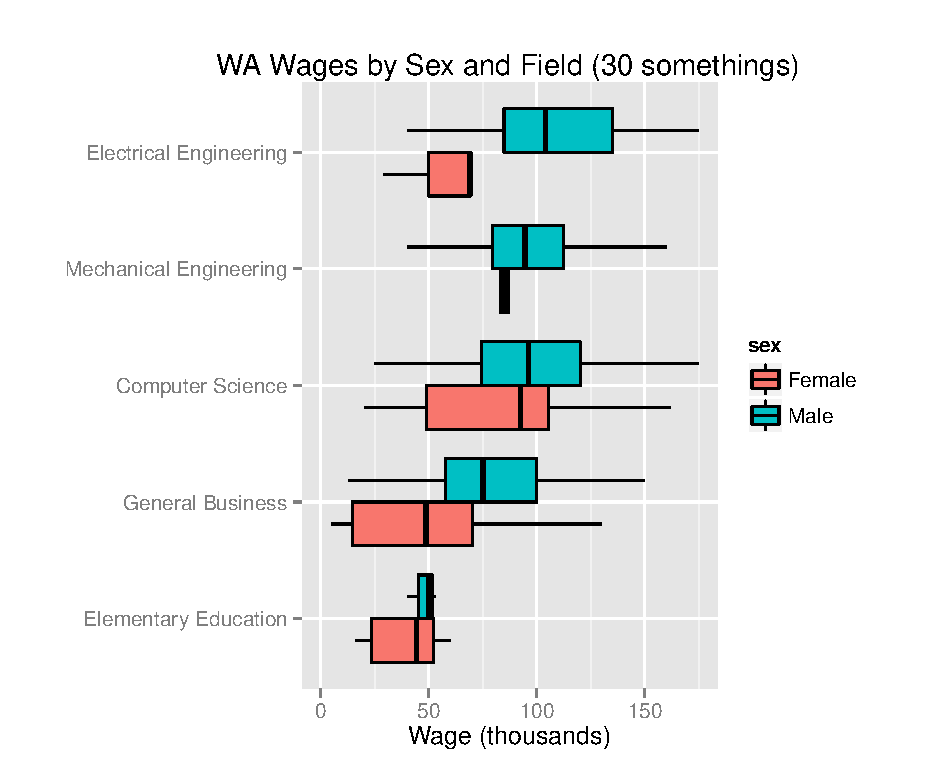
\includegraphics{figures/wa_30s_by_field_and_sex.eps}
    \caption{ Thirty to forty year old men make more than similar women }
  \end{figure}

  \begin{figure}[H]
    \centering
    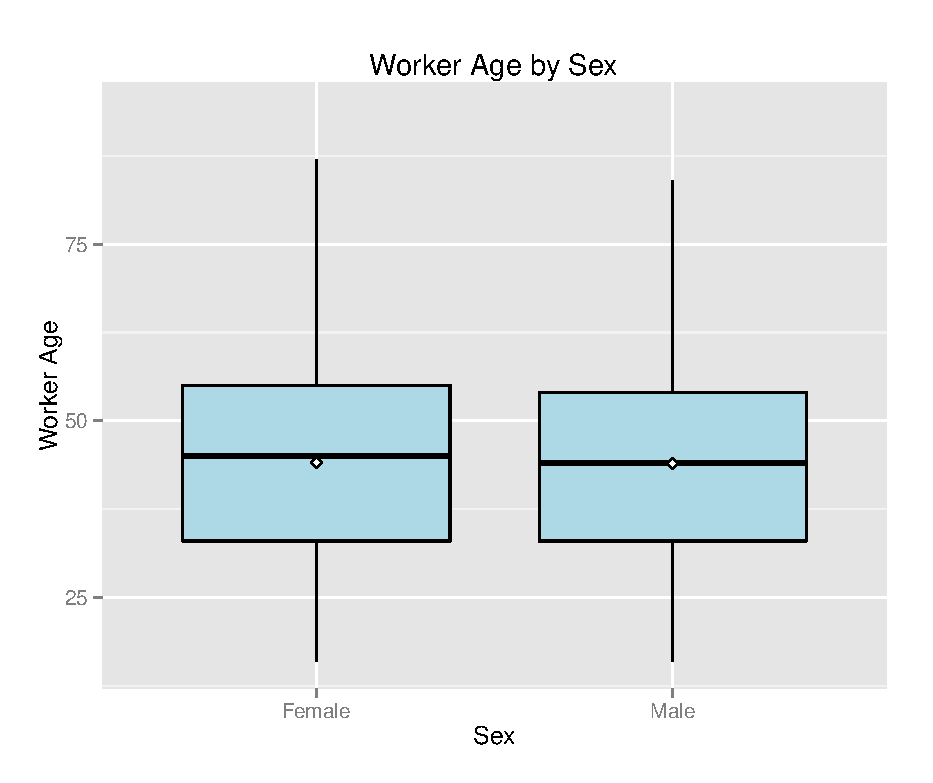
\includegraphics{figures/wa_age_by_sex.eps}
    \caption{Women workers are about the same age as men workers.}
  \end{figure}

  \begin{table}[ht]
    \centering
    \begin{tabular}{rlrrrrrr}
      \toprule
        & sex    & Min. & 1st Qu. & Median & Mean & 3rd Qu. & Max. \\
      \midrule
      1 & Female & 16   & 33      & 45     & 44   & 55      & 94 \\
      2 & Male   & 16   & 33      & 44     & 44   & 54      & 84 \\
      \bottomrule
    \end{tabular}
    \caption{Age by sex}
  \end{table}

  For low education workers, women tend to be older than men.  For high education workers, men
  tend to be older than men.  

  \begin{figure}[H]
    \centering
    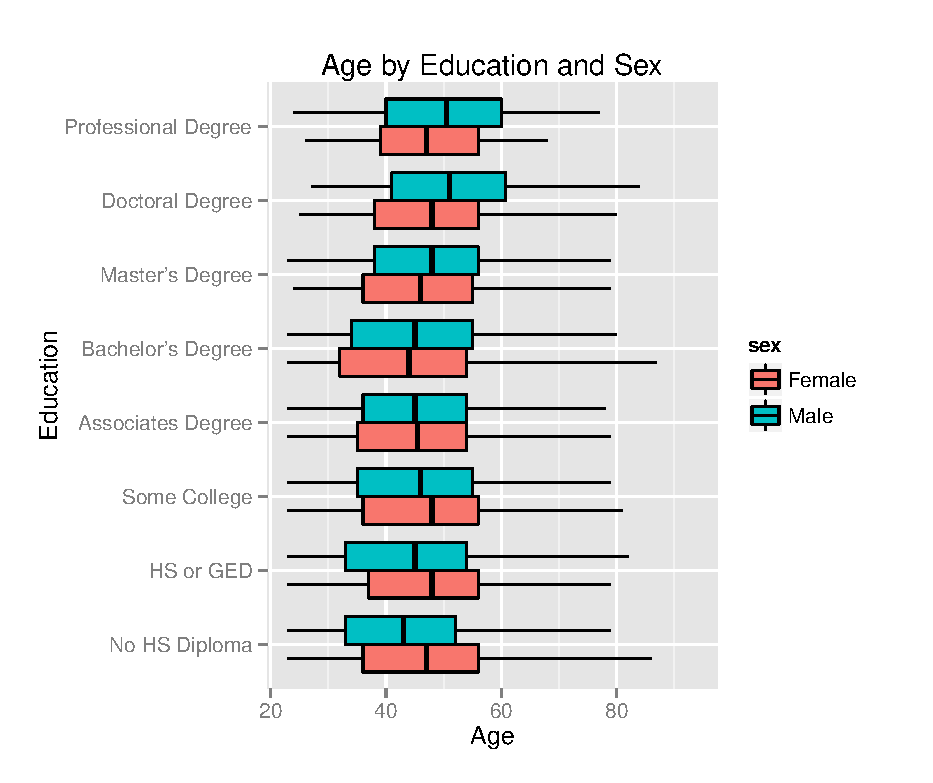
\includegraphics{figures/wa_age_by_education_and_sex.eps}
    \caption{WA wages by education and sex}
  \end{figure}

  \begin{itemize*}
    \item men with master's, etc. tend to move up into management. 

    \item women with master's, etc. tend to be married to men with similar education.  They may
      drop out of the workforce when they have kids.  They can afford to do this because of their
      high income spouses.

    \item women with little education need to work to pay for their kids

    \item women with little education need to work until they are fairly old to survive

  \end{itemize*}


\end{document}

